\section{Why Digital Predistortion?}
	
	Power amplifiers are used in almost all wireless communication devices. They amplify the communication signal such that a good signal to noise ratio is obtained. They also are an important power consuming block in a communication chain. A power amplifier is often operated in a nonlinear operation mode to improve its efficiency. This nonlinear behavior should be compensated to reach the strict telecommunication requirements.
	A Digital Pre-Distortion (DPD) is a common technique to linearise the input-output behavior of a power amplifier. With DPD the input signal of the amplifier is modified such that the desired (i.e. linear) behavior is obtained. 

	In this work a novel technique to design DPDs is presented. By first extracting the Best Linear Approximation (BLA) from input/output measurements of a nonlinear system, and consequently using the BLA with Iterative Learning Control (ILC), an effective compensation is possible. In this chapter, the theoretical background of BLA and ILC is discussed. This serves as an introduction to the main idea of this thesis : using these two techniques to design a DPD. 

\section{Current Techniques of DPD}
	\subsection{Direct and Indirect Learning}
	\subsection{Nonlinear Models}
	\subsection{Performance Assessment : Adjacent Channel Power Ratio}
\section{The Best Linear Approximation}

	\subsection{The Paradigm}

	Linear systems are completely characterised by their impulse response function. The knowledge of the impulse response function allows one to predict the output of the system, given any input. Nonlinear systems do not share this elegant property. Because nonlinear modelling can be quite involved and time-consuming, one can wonder if it is possible to construct a linear approximation that is `close enough' to the studied nonlinear system.

	The \emph{Best Linear Approximation} (BLA) is such an approximation. The BLA is a linear system that approximates the output of a nonlinear system with the response of a LTI model in mean square sense. The definition given below is in in time domain for ease of understanding. However, the BLA wil mainly be represented in the frequency domain which is a more convenient domain to study spectral regrowth.

	\begin{definition}
		The BLA of a nonlinear system is the linear system $G_{bla}(q)$ that minimizes the mean square error:
		
		\begin{align*}
		   G_{bla}(q) &= \underset{G(q)}{\text{arg min }} E \left\{ \left( \tilde{y}(n) - G(q)\tilde{u}(n)\right)^2 \right\}, \\
		   \tilde{u}(n) &= u(n) - E\{u(n)\},\\
		   \tilde{y}(n) &= y(n) - E\{y(n)\},\\
		\end{align*}

		Where $n$ is the time index, $q$ is the time shift operator ($qx(n) = x(k+1)$) and the expected value $E\{.\}$ is taken with respect to the random realisations of $u(n)$. Zero-mean input/output signals will be assumed from now on and thus the tilde symbol will be left out.
	\end{definition}

 Unlike the impulse response of a linear system, the BLA depends on the probability density function and power spectrum of the chosen input signal. The chosen class of signals in this work are excitations with a Gaussian pdf. The power spectrum is a design choice specific to each application. More specifically, random phase multisines will be used. These are periodic signals consisting of a sum of sines with a random phase, which have very nice properties to measure the BLA.
	\begin{definition}
	A multisine $u(t)$ can be defined in continuous time as : 
	\begin{align}
		u(t) = \sum^{N-1}_{k = 0}| A_k| cos(2\pi f_0t + \phi_k)
	\end{align}
	And computed in discrete time with the inverse discrete-time fourier transform :
	\begin{align}
		u_d(n) = \sum^{N-1}_{k = 0} |A_k| e^{j\phi_k} e^{jn\frac{k}{N}}
	\end{align}
		Where $A_k$ is the amplitude spectrum of the multisine and $\phi_k$ is the phase, chosen such that $E\{e^{j\phi_k}\} = 0$. $f_0$ is called the frequency resolution.
	\end{definition}
	
	The BLA allows to represent the output of a nonlinear system in the frequency domain as the sum of a linear contribution and a nonlinear distortion term $Y_s(k)$.
	
	\begin{align}
		Y(k) &= G_{bla}(k)U(k) + Y_s(k)	
	\end{align}
	
	Interestingly, $Y_s(k)$ is asymptotically zero-mean normally distributed. The variance of $Y_s(k)$ is a thus an useful measure for the quality of the linear approximation. To have a relative measure of the quality of approximation, the variance of $\frac{Y_s(k)}{U(k)}$ is often considered, and called the nonlinear stochastic variance of $G_{bla}(k)$.

	As a concluding but very  important remark: the BLA is only fit approximate PISPO (Period In, Same Period Out) systems meaning that the input and output signals have the same period length. An in-depth and more rigourous study of the BLA paradigm can be found in \cite{sysid}.

	\subsection{Detection of Nonlinear Distortions}

	Now the BLA has been defined, one wants to estimate it from input/output measurements.

	\subsubsection{Coherent Contributions}

%	Frequency combination is an interesting result that follows from Volterra nonlinear system theory : the frequency response at the output of a system $Y(\omega)$ is dependent on multiple input frequencies. 
	A coherent contribution is a contribution to the output spectrum $\phase{Y(\omega)}$ of a nonlinear system where the phase shift between input and output is constant, and can be modelled as a linear contribution. 
	Because the input signals are random phase multisines, all contributions that are non-coherent will have a random phase shift. Because $E\{e^{j\phi_k}\} = 0$, if different multisines are fed to the system and the output spectrum is averaged over these different realisations, non-coherent contributions will be averaged to zero. This last properties is at the core of the robust measurement method that is presented in the next section.

	\subsubsection{Robust Measurement Approach }

	To measure the BLA, one can measure  the steady-state response over $P$ periods of $M$ multisines with different random phase realisations. Because of previous properties, the sample variance over the P periods only depends on the output noise, while the sample variance over the M realisations depends on both the stochastic nonlinear distortions and the output noise. This allows to discriminate between nonlinear distortions and noise, and to measure the BLA. Figure \ref{fig:robustMt} shows a visual aid to understand the measurement method. Choosing a high $M$ decreases the nonlinear distortion variance and increasing $P$ decreases the noise variance. This is the only measurement method that will be used in this work.

	\begin{figure}[hbtp]
	\centering
		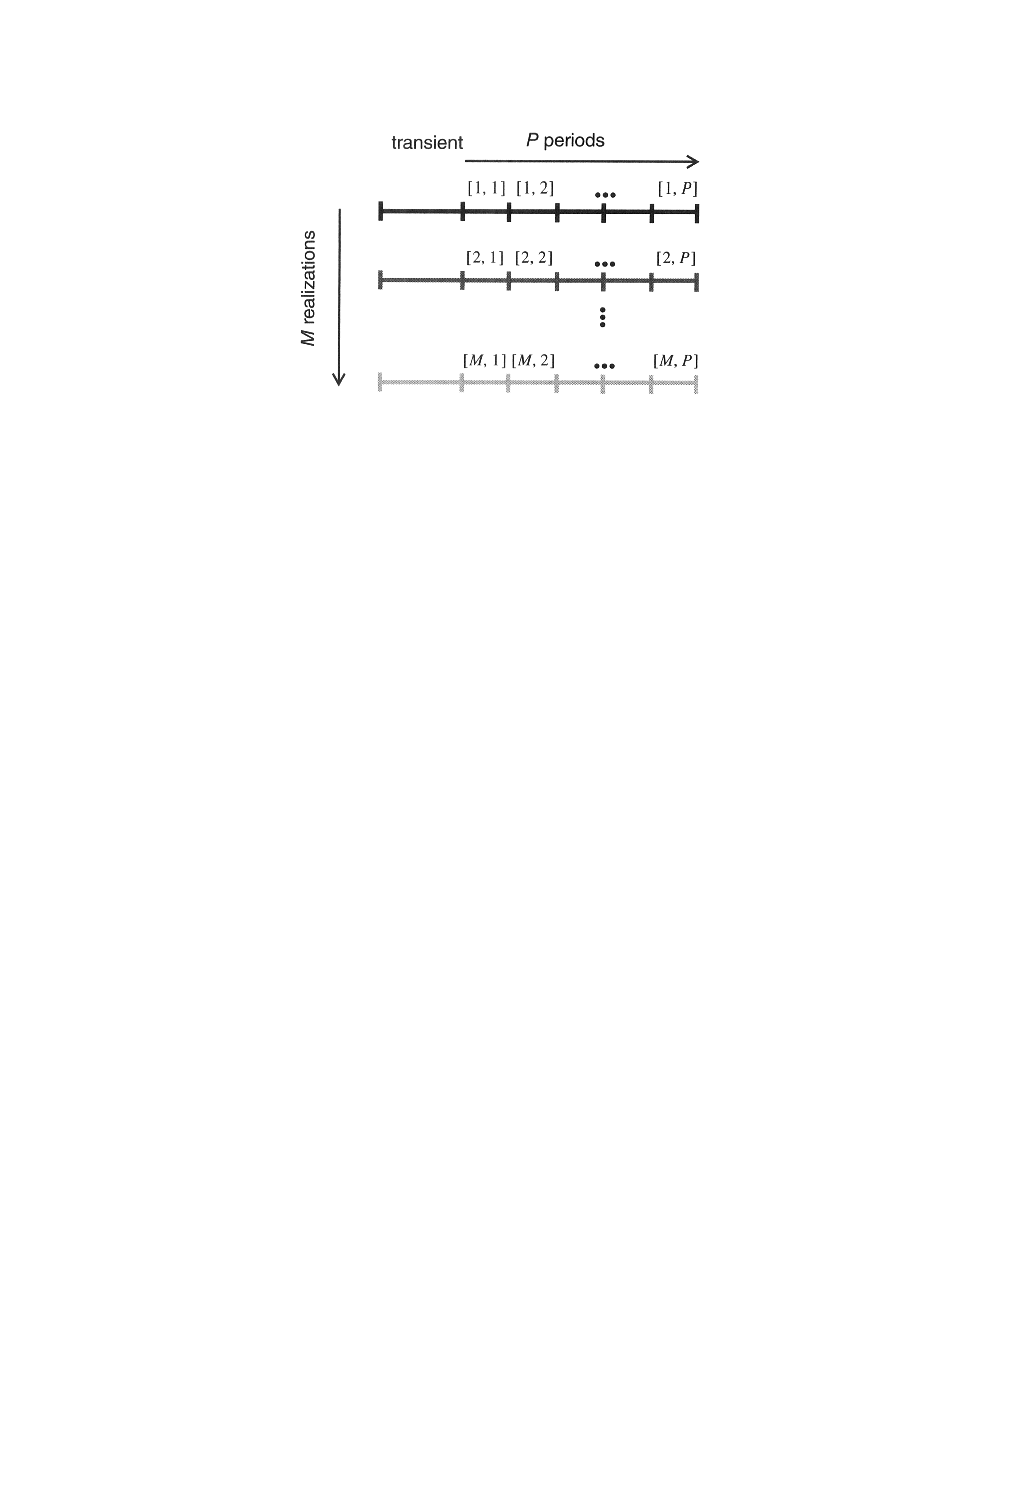
\includegraphics[width=0.5\linewidth]{images/robustMt.pdf}
		\caption{The robust measurement procedure. Averaging i/o spectra over periods at each realisation gives an estimated FRF $\hat{G}_m$ and an estimate for the noise variance $\hat{\sigma}_{n,m}$. Further averaging over the realisations gives an estimate of the nonlinear variance $\hat{\sigma}_s$, and an improved noise variance $\hat{\sigma}_{n}$.}
		\label{fig:robustMt}
	\end{figure}

	\subsection{Out of Band BLA and the Tickler Tone}
	
	A nonlinear system will 

	
\section{Iterative Learning Control}
	\subsection{The Algorithm}
	\subsection{Properties}